\documentclass[tikz,border=12pt]{standalone}
\usepackage{tikz}
\usetikzlibrary{positioning, arrows.meta, fit, backgrounds, calc}

%% ── Colours ─────────────────────────────────────
\definecolor{cExt}{RGB}{20,184,166}   % teal   – external
\definecolor{cFE} {RGB}{59,130,246}   % blue   – frontend
\definecolor{cGW} {RGB}{168,85,247}   % purple – gateway
\definecolor{cBE} {RGB}{16,185,129}   % green  – backend
\definecolor{cDB} {RGB}{245,158,11}   % amber  – database
\definecolor{cST} {RGB}{239,68,68}    % red    – storage
\definecolor{cMO} {RGB}{107,114,128}  % gray   – monitoring

\tikzset{
  %% parametric coloured box
  B/.style={rectangle, rounded corners=5pt, draw=#1!65, fill=#1!10,
            line width=0.8pt, minimum width=2.8cm, minimum height=0.82cm,
            font=\small\bfseries, text=#1!80, align=center},
  %% small module inside backend group
  M/.style={rectangle, rounded corners=3pt, draw=#1!55, fill=#1!8,
            line width=0.6pt, minimum width=2.05cm, minimum height=0.65cm,
            font=\scriptsize\bfseries, text=#1!80, align=center},
  %% arrows
  A/.style ={-{Stealth[length=5pt,width=4pt]}, line width=1pt,   color=#1},
  DA/.style={-{Stealth[length=5pt,width=4pt]}, line width=0.8pt, dashed, color=#1},
  %% group rectangle
  GRP/.style={rectangle, rounded corners=8pt, draw=#1!35, fill=#1!5,
              line width=1pt, inner sep=10pt},
}

\begin{document}
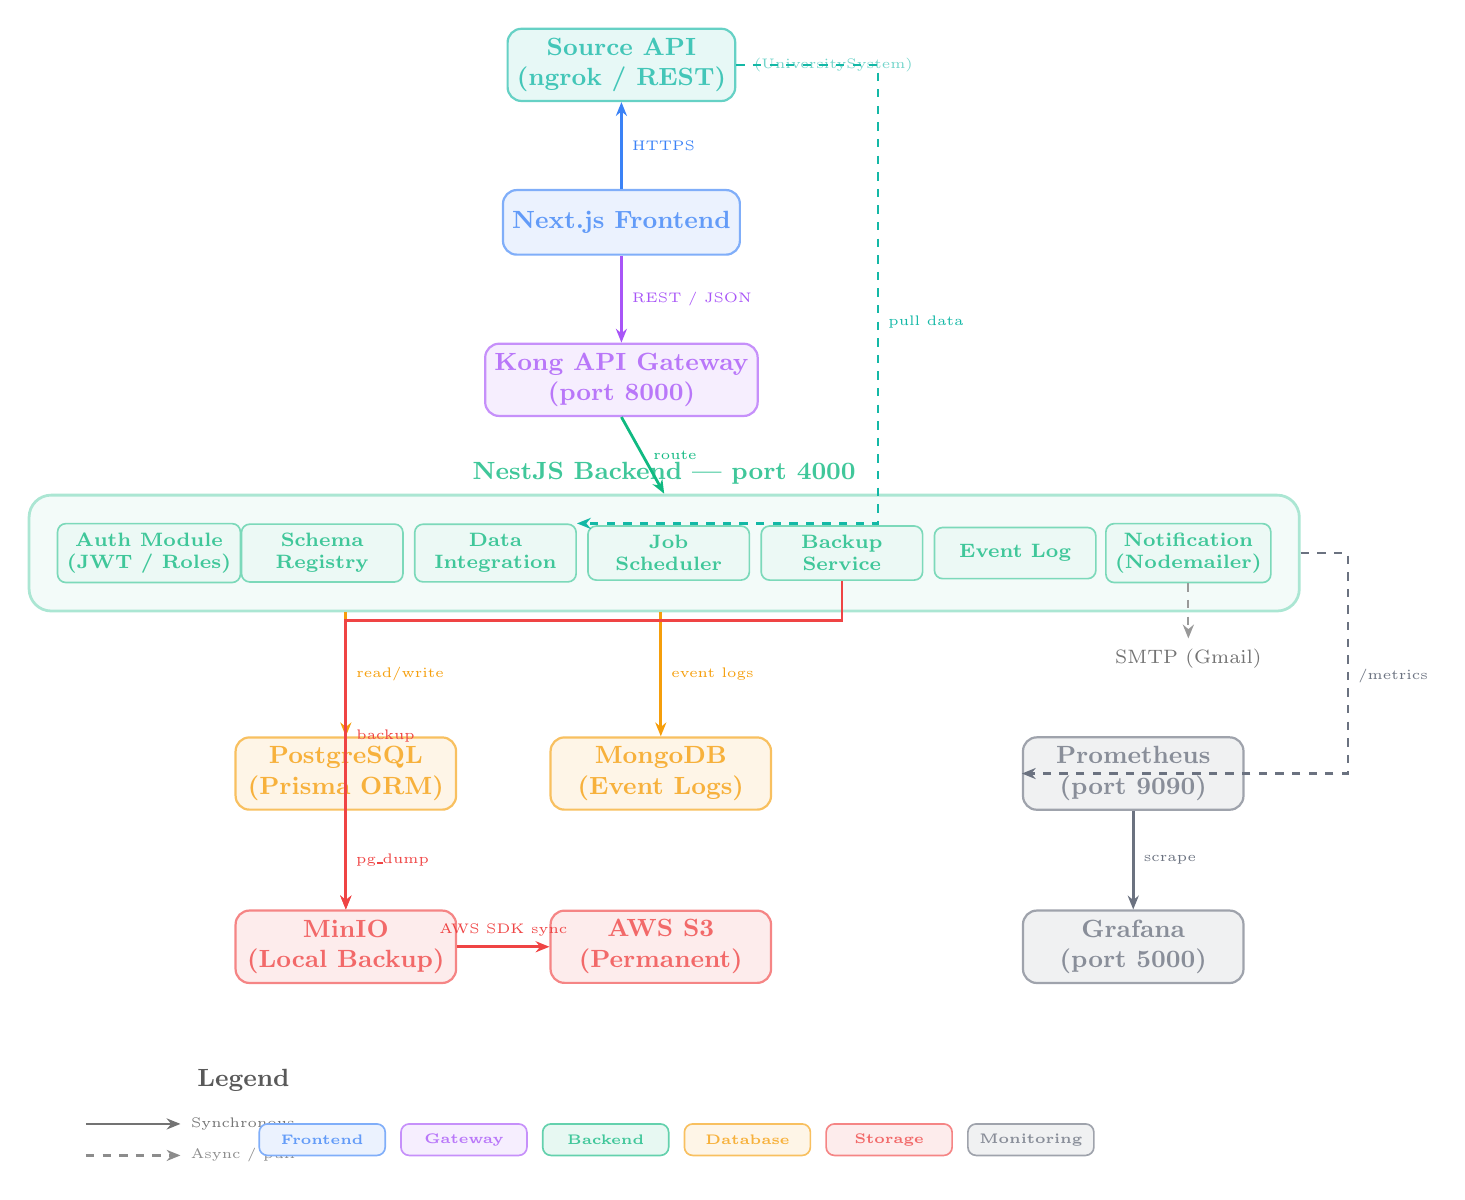
\begin{tikzpicture}

%% ════════════════════════════════════════════════
%%  NODES  (absolute coordinates for full control)
%% ════════════════════════════════════════════════

%% External source  – top centre
\node[B=cExt] (src)  at (7, 14)   {Source API\\(ngrok / REST)};

%% Frontend
\node[B=cFE]  (fe)   at (7, 12)   {Next.js Frontend};

%% Kong
\node[B=cGW]  (kong) at (7, 10)   {Kong API Gateway\\(port 8000)};

%% ── Backend modules  (y = 7.8, evenly spaced) ──
%%    x positions: 1, 3.2, 5.4, 7.6, 9.8, 12.0, 14.2
\node[M=cBE] (auth)  at (1.0,  7.8) {Auth Module\\(JWT / Roles)};
\node[M=cBE] (sch)   at (3.2,  7.8) {Schema\\Registry};
\node[M=cBE] (di)    at (5.4,  7.8) {Data\\Integration};
\node[M=cBE] (sched) at (7.6,  7.8) {Job\\Scheduler};
\node[M=cBE] (bak)   at (9.8,  7.8) {Backup\\Service};
\node[M=cBE] (el)    at (12.0, 7.8) {Event Log};
\node[M=cBE] (notif) at (14.2, 7.8) {Notification\\(Nodemailer)};

%% Backend group box (drawn behind modules)
\begin{scope}[on background layer]
  \node[GRP=cBE,
        fit=(auth)(sch)(di)(sched)(bak)(el)(notif),
        label={[font=\small\bfseries,text=cBE!80]above:NestJS Backend — port 4000}
       ] (be) {};
\end{scope}

%% ── Databases  (y = 5) ──
\node[B=cDB] (pg)  at (3.5, 5)  {PostgreSQL\\(Prisma ORM)};
\node[B=cDB] (mg)  at (7.5, 5)  {MongoDB\\(Event Logs)};

%% ── Storage  (y = 2.8) ──
\node[B=cST] (minio) at (3.5, 2.8) {MinIO\\(Local Backup)};
\node[B=cST] (s3)    at (7.5, 2.8) {AWS S3\\(Permanent)};

%% ── Monitoring  (far right, clear of everything) ──
\node[B=cMO] (prom)  at (13.5, 5)   {Prometheus\\(port 9090)};
\node[B=cMO] (graf)  at (13.5, 2.8) {Grafana\\(port 5000)};

%% ════════════════════════════════════════════════
%%  ARROWS — top section
%% ════════════════════════════════════════════════

%% User (implicit) → Source API label
\node[font=\tiny, cExt!60, right=0.1cm of src] {(University\\System)};

%% Source API ↔ Frontend (user flow)
\draw[A=cFE]  (fe.north)   -- node[right,font=\tiny]{HTTPS} (src.south);

%% Frontend → Kong
\draw[A=cGW]  (fe.south)   -- node[right,font=\tiny]{REST / JSON} (kong.north);

%% Kong → Backend
\draw[A=cBE]  (kong.south) -- node[right,font=\tiny]{route} (be.north);

%% Source API --pull--> Data Integration  (dashed, avoids centre by going right side)
\draw[DA=cExt]
  (src.east) -- ++(1.8,0)
              |- node[right,font=\tiny,pos=0.28]{pull data}
              (di.north east);

%% ════════════════════════════════════════════════
%%  ARROWS — Backend → Databases
%%  Strategy: one clean vertical drop from the point
%%  on be.south directly above each target.
%%  be.south -| pg.north  =  same x as pg.north, y of be.south
%% ════════════════════════════════════════════════

%% → PostgreSQL  (label: auth / schema / data integration write here)
\draw[A=cDB]
  (be.south -| pg.north) -- node[right,font=\tiny]{read/write} (pg.north);

%% → MongoDB  (label: scheduler + event log write here)
\draw[A=cDB]
  (be.south -| mg.north) -- node[right,font=\tiny]{event logs} (mg.north);

%% ════════════════════════════════════════════════
%%  ARROWS — Storage
%% ════════════════════════════════════════════════

%% Backup Service → MinIO  (vertical, then bend left)
\draw[A=cST]
  (bak.south) -- ++(0,-0.5)
               -| node[right,font=\tiny,pos=0.7]{backup} (minio.north);

%% PostgreSQL → MinIO  (straight down)
\draw[DA=cST]
  (pg.south) -- node[right,font=\tiny]{pg\_dump} (minio.north);

%% MinIO → S3  (horizontal)
\draw[A=cST]
  (minio.east) -- node[above,font=\tiny]{AWS SDK sync} (s3.west);

%% ════════════════════════════════════════════════
%%  ARROWS — Monitoring  (all on the right, no overlap)
%% ════════════════════════════════════════════════

%% Backend.east → Prometheus
\draw[DA=cMO]
  (be.east) -- ++(0.6,0)
              |- node[right,font=\tiny,pos=0.28]{/metrics} (prom.west);

%% Prometheus → Grafana
\draw[A=cMO]
  (prom.south) -- node[right,font=\tiny]{scrape} (graf.north);

%% ════════════════════════════════════════════════
%%  Notification → SMTP  (below, far right — isolated)
%% ════════════════════════════════════════════════
\draw[DA={black!40}]
  (notif.south) -- ++(0,-0.7)
  node[below,font=\scriptsize,black!55]{SMTP (Gmail)};

%% ════════════════════════════════════════════════
%%  LEGEND
%% ════════════════════════════════════════════════
\begin{scope}[shift={(0, 1)}]
  \node[font=\small\bfseries, black!65] at (2.2, 0.1) {Legend};

  \draw[A={black!55}]  (0.2,-0.45) -- (1.4,-0.45)
       node[right,font=\tiny]{Synchronous};
  \draw[DA={black!45}] (0.2,-0.85) -- (1.4,-0.85)
       node[right,font=\tiny]{Async / pull};

  \foreach \c/\t/\x in {
    cFE/Frontend/3.2, cGW/Gateway/5.0,
    cBE/Backend/6.8,  cDB/Database/8.6,
    cST/Storage/10.4, cMO/Monitoring/12.2}
  {
    \node[rectangle, rounded corners=3pt,
          draw=\c!65, fill=\c!10, line width=0.6pt,
          minimum width=1.6cm, minimum height=0.4cm,
          font=\tiny\bfseries, text=\c!80]
      at (\x,-0.65) {\t};
  }
\end{scope}

\end{tikzpicture}
\end{document}
